\chapter{Introduction}
\label{chap:introduction}


Traffic congestion in urban areas became a bigger problem every year in the past decades. Increasing traffic causes several issues, for example high monetary and environmental costs due to gasoline consumption and by emitting $CO_2$ to the environment. There are several strategies to reduce urban traffic to mitigate these problems like for example new investments in public transport infrastructure. However, according to a study by Hao et al. \cite{HAO2016121}, car sales will continue to grow in the upcoming decades and therefore also traffic will continue to become worse in big cities. Thus, it is important to find ways to reduce traffic in urban areas.

With more vehicles driving in urban areas, there also comes the need for a sufficient number of parking spaces. Finding parking spaces in urban areas can be really difficult, frustrating and time consuming. There often exists some information about the availability of parking spaces in parking garages, but in most cities the situation of road side parking is unknown. This not only leads to frustrated drivers, who are searching for parking spaces a long time, but again contributes to urban traffic congestion as many cars have to drive around close to their destination while searching for free parking spaces. 

There are many studies, which show that the searching for parking spaces adds a lot of traffic. A study by Nawaz et al. \cite{Nawaz:2013:PSB:2500423.2500438} shows that about 30\% of traffic congestion is created by drivers looking for free parking spaces. Another study \cite{TexasMobilityReport} concludes that alone in 2007 searching for parking spaces caused costs of about 78 billion US dollars by using 2.9 billion gallons of wasted gasoline and 4.2 billion lost hours only in the United States. Furthermore, cruising causes a lot of greenhouse emissions which is not only bad for the environment and contributes to climate change, but also lowers the quality of living in big cities through the significant amount of air pollution.

One of the most important contributors to long search times for parking spaces is not only the lack of vacant parking spaces, but also the lack of information about free parking spaces. Therefore, one way to mitigate many of the above stated problems is to determine the current parking space situation in the city and make it accessible to the public (for instance via a Web application), so that drivers can efficiently navigate to a vacant parking space, or even decide if they want to go by car or use public transportation, depending on the number of parking spaces available close to their destination. 

%TODO




Yet, detection of road side parking spaces and their states is a challenging task. Of course an obvious approach to the problem would be to put stationary sensors to every parking space in the city, which check, if the corresponding parking space is occupied or vacant. This, however, has the drawback to be very expensive as, for big cities, thousands of sensors would have to be bought, installed, and maintained. Moreover, because the state of parking parking spaces does not often change, the high frequency of sensing with such a system would be rather inefficient.





\section{Drive-By Parking Space Sensing}

A promising novel approach to sense a city's parking situation is the use of mobile sensors instead of static ones. Several prototypes, including the ParkNet prototype by Mathur et al. \cite{Mathur:2010:PDS:1814433.1814448}, which will be discussed later on, show that mobile crowd sensing has the advantage to be usually more cost effective and can provide sufficient accuracy for the purpose of providing parking space availability maps. 

This thesis will focus on "drive-by park sensing". The idea of drive-by approaches is that there are sensing vehicles which are driving through the city and collecting data of their environment through mounted sensors. Using the collected data, parking cars and vacant parking spaces can be detected. There already exists a prototype implementation of such a system. In 2010, Mathur et al. \cite{Mathur:2010:PDS:1814433.1814448} presented their system, called ParkNet, which continuously measures the distance to the nearest obstacle on the side of the road, as well as the location of the sensing vehicle through a GPS sensor. Using these data, they used a distance threshold to detect parking cars and vacant parking spaces. A more detailed description of their work can be found in section \ref{sec:related_driveby_park_sensing_distance}.

Figure \ref{fig:driveby_standard_parking_situation} shows a standard drive-by scenario of a sensing vehicle that passes two parallel parked cars and a vacant parking space in between them. The distance measurements while passing the parked cars will be much shorter than the measurements taken while passing the vacant parking space. This should allow a basic algorithm to recognize parking cars and vacant parking spaces.

\begin{figure}
	\centering
	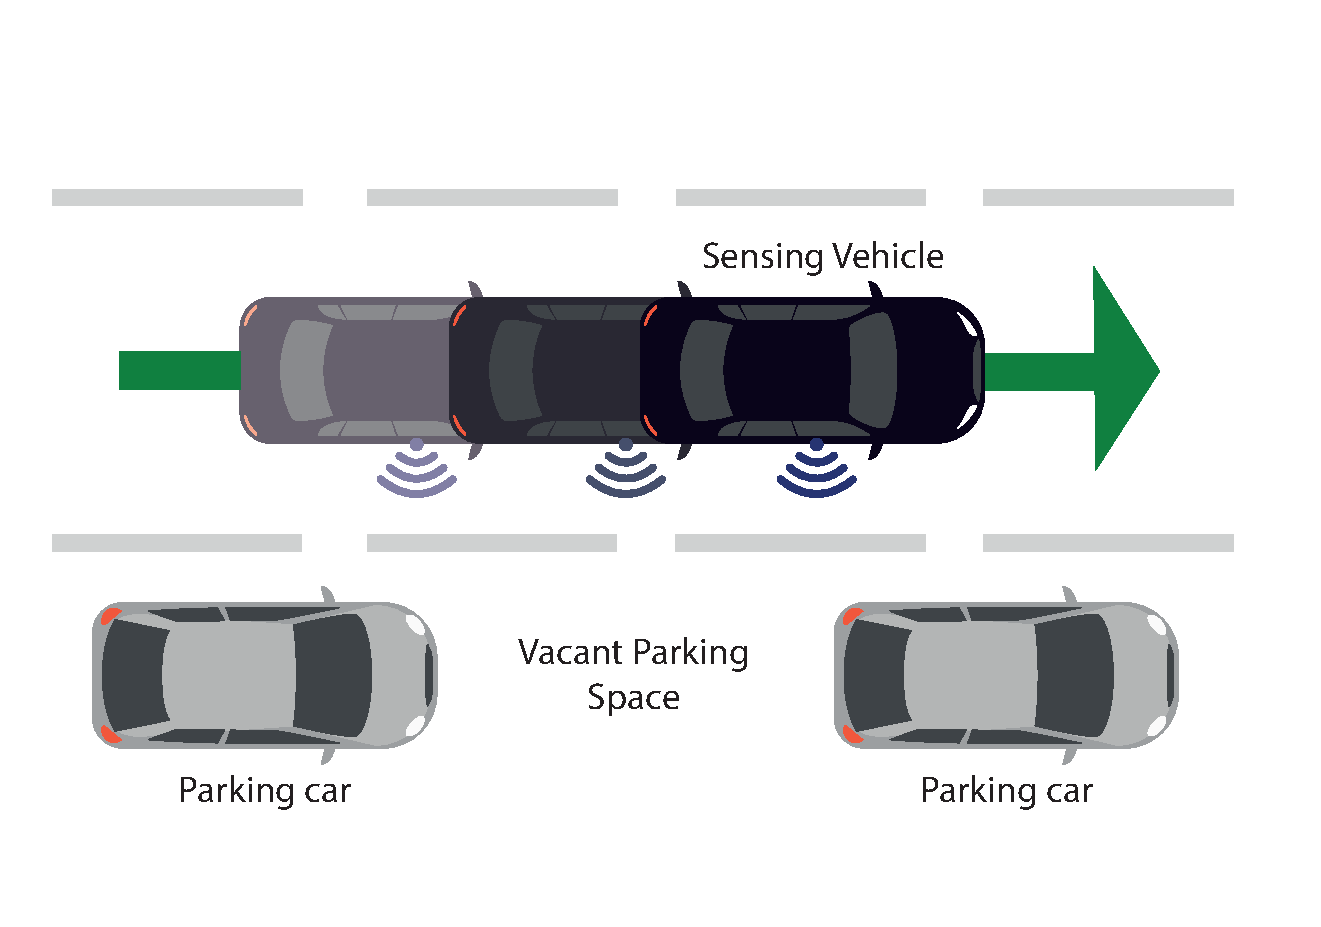
\includegraphics[width=0.9\textwidth]{img/drive-by-parking-situation-pictogram.eps}
	\caption{The sensing vehicle passes two parked cars and should identify a vacant spot in between using distance and location measurements.}
	\label{fig:driveby_standard_parking_situation}
\end{figure}

However, the situation shown in Figure \ref{fig:driveby_standard_parking_situation} is an idealistic one. In real life traffic, there will be much more complex situations to face, which are not as easily detectable and which might influence the success of the detection. For instance, the sensing vehicle might not drive in the right-most lane, therefore the measured distances will be much longer. Another possible issue are other driving cars, motorcycles or bicycles which the sensing car overtakes. Many of such distractions have to be filtered out to counteract false detection results.
%The existing ParkNet prototype does not take any of such situations into account, because it was only evaluated on parallel parking cars on single lane roads.

The high complexity of urban traffic and the many distractions during sensing make it nearly impossible to create a rule set based on the sensor measurements which would be able to detect parking situations at a sufficient accuracy. Therefore, simple thresholding will not work in real life traffic scenarios. Furthermore, such rule sets would have to be created for each city individually because of the different nature of the roads and the parking spaces. For instance, the distance between lanes and parking spaces can vary highly in two different cities. Thus, to be able to detect parking situations, new methods have to be found, that are more flexible to distractions and changes in the environment.

%There are several approaches to mobile parking availability sensing, which will be discussed in chapter \ref{chap:relatedwork}. In this thesis a "drive-by park sensing" approach will be implemented, tested and evaluated. The approach works as follows: Several sensing vehicles drive through the city and measure their environment using two sensors. The first sensor measures the distance to the nearest obstacle on the right side of the road (often a parking car). A LIDAR (Light Detection and Ranging) sensor is being used to measure the distance, because of its high range and high measuring frequency. The second sensor is a GPS sensor which tracks the position of the vehicles. So while the vehicles are driving through the city, both sensors are constantly recording their environment. Using these data parking cars should be detected and vacant parking spaces should be derived using parking space maps.

%Figure \ref{fig:driveby_standard_parking_situation} shows a standard scenario of a sensing vehicle which passes two parallel parked cars and a vacant parking space in between them. The distance measurements while passing the parked cars will be much shorter than the measurements taken while passing the vacant parking space. This should allow a basic algorithm to recognize parking cars and vacant parking spaces.

%\begin{figure}
%	\centering
%	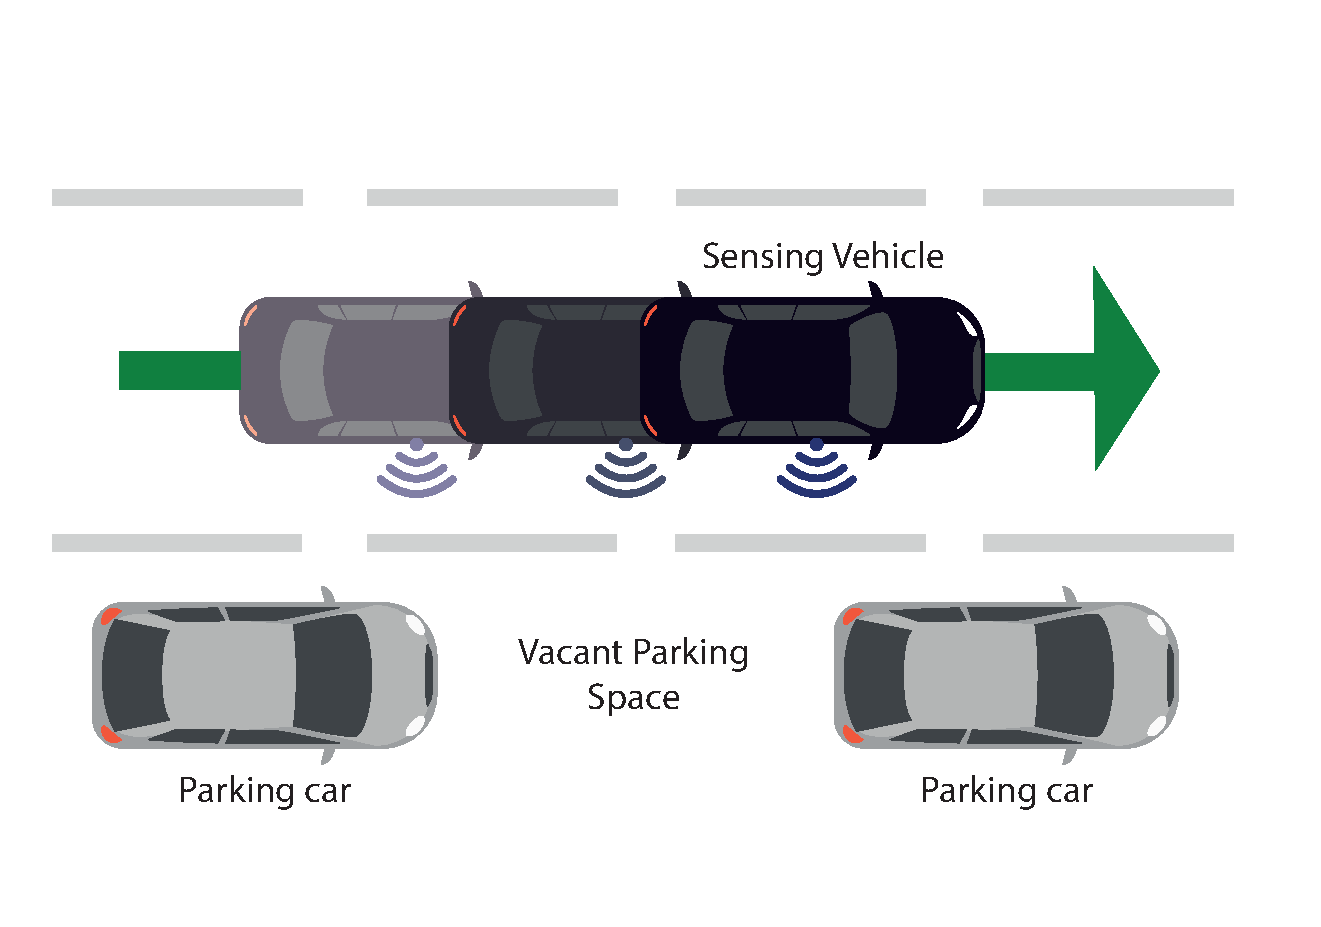
\includegraphics[width=0.9\textwidth]{img/drive-by-parking-situation-pictogram.eps}
%	\caption{The sensing vehicle passes two parked cars and should identify a vacant spot in between using distance and location measurements. \todo{Hier Referenz zu Parknet-Paper??? Ähnliche Grafik...}}
%	\label{fig:driveby_standard_parking_situation}
%\end{figure}

%However, the situation which is shown in figure \ref{fig:driveby_standard_parking_situation} is an idealistic one. In real life traffic, there will be much more complex situations to face, which are not as easily detectable and which might influence the success of the detection. For instance, the sensing vehicle might not drive in the right-most lane, therefore the measured distances will be much longer. Another possible issue are other driving cars, motorcycles or bicycles which the sensing car overtakes. There are many of such distractions which have to be filtered out to ensure that there are as few false detections as possible. 

%The high complexity of urban traffic and the many distractions during sensing make it nearly impossible to create a rule set based on the sensor measurements which would be able to detect parking situations at a sufficient accuracy. Furthermore, such rule sets would have to be created for each city individually because of the different nature of the roads and the parking spaces. For instance, the distance between roads and parking spaces can vary highly between two cities. In this thesis several machine learning techniques are being tested and compared to each other to find out if machine learning can be used to identify complex road side parking situations, to filter out distractions like overtaking situations and to detect vacant parking spaces. 

%During test runs with a prototype car in Linz, Austria, sample measurements are being recorded, where the focus lies on creating very diverse and realistic situations. The recorded data is being filtered and pre-processed before it is used as input for the machine learning algorithms. 

\section{Research goals}

The overall goal of this thesis is to determine which accuracy can be achieved for detecting the parking space situation in urban real world traffic scenarios using drive-by park sensing on multi lane streets. More specific goals are described below:

\begin{description}

\item[Obtaining an own dataset of different drive-by scenarios.] A testbed should be built which can be mounted on a standard car. This testbed should collect sensor values of a distance sensor as well as a GPS receiver during test drives in the city of Linz, Austria. Furthermore, the test bed should also capture images to record the ground truth of the sensed scenes.

\item[Estimating parking availability using machine learning.] Using the acquired dataset, objects, like parking cars, should be detected and classified. The use of machine learning and deep learning approaches to do so should be evaluated and with the
help of parking space maps the count of vacant parking spaces and their location should be derived.

\item[Identifying sensing distractions.] There are many scenarios in which the drive-by park sensing will not work as expected. For example, when the sensing vehicle overtakes another driving car, it cannot detect the parking cars behind. Such situations
should be detected and classified as distractions.

\item[Deriving basic parking space maps.] Parking space maps are necessary for the overall system to work as only using the sensor data it is not possible to determine if it is legal to park at a certain location. As there are no parking space maps with sufficient quality available at city authorities, a basic parking space map should be derived using the acquired dataset.

\end{description}




\section{Research methodology}
To determine if it is possible to derive parking availability statistics from drive-by sensing in complex road scenarios several steps have to be taken. First, a test bed has to be build which is able to access the distance and GPS sensors and which records these data continuously while driving by. The detailed description of all hardware parts will be given in section \ref{sec:testbed} \todo{ref}. The test bed and all sensors will be mounted on a typical car and during test drives in Linz, Austria raw sensor data will be collected from all sensors. The variability of situations in the collected data is of great importance as the goal of this thesis is to investigate the use of a drive-by sensing system in complex traffic scenarios. A detailed description about recording the dataset will be given in
section \todo{ref} \ref{sec:dataset}.

After a big enough dataset has been acquired, the sensor data is preprocessed and outliers are being filtered out. Furthermore, the sensor measurements are being segmented, so that measurements belonging to the same object (e.g parking car) are treated as one segment. This process will be described in more detail in section \todo{ref} \ref{sec:segmentation}. Features on the given segments are calculated (for example the length of the segments and the distance to the right side of the road) and are used as input for several machine learning techniques which will be compared against each other in terms of accuracy. Additionally, some deep learning models will be evaluated and their performance will be evaluated as well. The description of the machine learning  models and the experiments can be found in section \todo{ref} \ref{sec:experiments} and the results and comparison of all approaches is described in section \todo{ref} \ref{sec:results}. \todo{update :)}



\section{Envisioned Parking Information System}

%The proposed system is using a crowd sensing approach containing several mobile sensors in the form of sensing vehicles which sense the current parking availability situation. 

Figure \ref{fig:envisioned_system} shows an overview of how the proposed drive-by sensing system could work. On the left, a scene of urban streets is depicted, where cars are parking beside the road and sensing vehicles detect parking cars while they are driving by. The sensing vehicles operate by using an optical distance sensor which is continuously measuring the distance to the nearest obstacle on the right side of the road. Furthermore, a GPS receiver determines the corresponding position. This information is used for the analysis of the parking situation, so that parking cars and vacant parking spaces are being detected.

The parking situation analysis can be performed by each sensing vehicle for itself. After obtaining the results, all the derived information may be sent to central server, which then combines the data of all sensing vehicles and computes a parking availability map. This map of free and occupied parking spaces can then be used for showing users the current parking situation (e.g. through a web application) so that they can decide if they want to go by car or by public transport. Furthermore, the information of vacant parking spaces could be used effectively by GPS navigation systems which could direct the driver to a vacant parking space close to his end destination and therefore maybe prevent long parking search times.


\begin{figure}
	\centering
	\includegraphics[width=\textwidth]{img/envisioned-system.eps}
	\caption{Envisioned system of several vehicles driving through the city and sensing its parking availability situation}
	\label{fig:envisioned_system}
\end{figure}
